\documentclass[12pt]{article}
\usepackage{import}
\usepackage[scaled]{helvet}
\usepackage[T1]{fontenc}
\renewcommand\familydefault{\sfdefault} 
\usepackage{rotating}
\usepackage{natbib}
\usepackage{soul}
\bibliographystyle{agsm} %Imperial College Harvard Style
\usepackage{authblk} %Add second authors and affiliations
\renewcommand{\bibsection}{} %Hide 'References' header
\renewcommand{\abstractname}{Summary}
\usepackage{float}
\usepackage{graphicx}
\usepackage{mathtools}
\usepackage{amsmath}
\usepackage{setspace}
\usepackage[font=singlespacing]{caption}
\usepackage{listings}
\lstset{keywordstyle=\bfseries, breaklines=true,
postbreak=\mbox{\textcolor{red}{$\hookrightarrow$}\space}, basicstyle=\footnotesize, numbers=left,
stepnumber=1, numberstyle=\tiny}
\usepackage[usenames,dvipsnames, table, xcdraw]{xcolor}
\usepackage{multirow}
\definecolor{mygray}{gray}{0.1}
\definecolor{blue(pigment)}{rgb}{0.2, 0.2, 0.6}
\usepackage[left=2cm,right=2cm,top=2.5cm,bottom=2cm, headheight=15pt]{geometry}
\usepackage{tikz}
\usetikzlibrary{arrows, positioning, shapes.geometric}
\usepackage{hyperref}
\renewcommand{\figurename}{Figure}
\renewcommand{\thefigure}{S\arabic{figure}}

\renewcommand{\tablename}{Table}
\renewcommand{\thetable}{S\arabic{table}}


\hypersetup{
         colorlinks=true,
         linkcolor=mygray,
         filecolor=magenta,
         urlcolor=mygray,
         citecolor=mygray,}

 %remove chapter text headers
\usepackage{titlesec}
\usepackage{ccaption}

%headers
\usepackage{fancyhdr}

\title{\textbf{Supplementary Information} 
}
\author{}
\date{}
\DeclareUnicodeCharacter{2212}{-}
\setcounter{tocdepth}{3}
\setcounter{secnumdepth}{3}

\begin{document}

\maketitle



\section{Methyl viologen treatment leads to enhanced light-dependent intracellular ROS accumulation}


\begin{figure}[H]
    \centering
    \includegraphics[width=\hsize]{../Figures/MV_adaptation/MV_ROS_DFCDA_Syn6803.png}
    \caption{ROS quantification assay based on the substrate DCFH-DA, which becomes fluorescent upon reaction with intracellular reactive oxygen species. A) DCF fluorescence in cultures of \textit{Synechocystis} at various time points after treatment with 10 $\mu$M methyl viologen (in the dark). B) DCF fluorescence at various time points after treatment with 10 $\mu$M MV (under 40 $\mu$mol$\cdot$m$^{-2}\cdot$s$^{-1}$ of white light illumination). C) Fold changes in DCF fluorescence between cultures treated with methyl viologen and no treatment control in the darkness and light at various time points. Error bars represent standard error of the mean from three biological replicates (individual colonies treated independently).}
    \label{fig:spectraMV1}
\end{figure}

\newpage

\section{Adaptation to methyl viologen is not due to its degration over time}

\begin{figure}[H]
    \centering
    \includegraphics[width=\hsize]{../Figures/MV_adaptation/growth_curves_firstevolution_Wt_6umMV.png}
    \caption{Growth curves of three independent unadapted (A) and MV-adapted (B) cultures of \textit{Synechocystis sp.} PCC 6803 growing at 30$^\circ$C under constant illumination (intensity = 100 $\mu$mol$\cdot$m$^{-2}\cdot$s$^{-1}$) in the absence (green trace) and upon addition of 6 $\mu M$  methyl viologen (from a fresh stock) during exponential growth (purple trace). Shaded regions represent standard errors over the means from three biological replicates.}
    \label{fig:freshstock}
\end{figure}


\begin{figure}[H]
    \centering
    \includegraphics[width=\hsize]{../Figures/MV_adaptation/spectra_endpoint_firstevolution_Wt_6umMV.png}
    \caption{Absorbance spectra of unadapted (A) and adapted (B) cultures of \textit{Synechocystis sp.} PCC 6803 after 6 days of growth at 30$^\circ$C under constant illumination (intensity = 100 $\mu$mol$\cdot$m$^{-2}\cdot$s$^{-1}$) in the absence (green trace) and upon addition  of 6 $\mu$M methyl viologen during mod-log phase (purple trace). Shaded regions represent standard errors over the means from three biological replicates.}
    \label{fig:spectraMV1}
\end{figure}


\section{Addition of methyl viologen at various growth phases}

\begin{figure}[H]
    \centering
    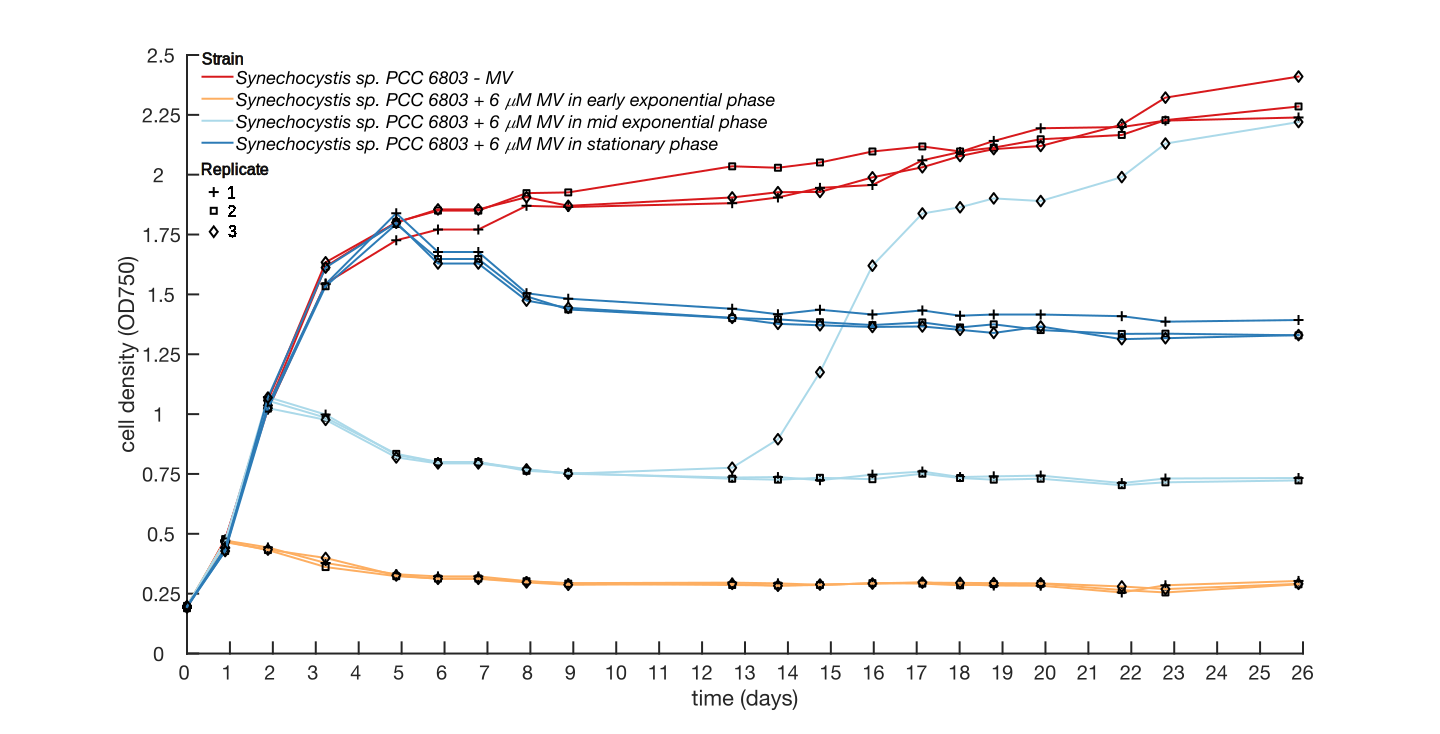
\includegraphics[width=\hsize]{../Figures/MV_adaptation/growthcurves_growthstages_Howe.pdf}
    \caption{Growth curves of \textit{Synechocystis sp.} PCC 6803 strains grown at 30 $^\circ$C under constant illumination (intensity = 40 $\mu$mol$\cdot$m$^{-2}\cdot$s$^{-1}$) in the absence (red trace) and upon addition  of 6 $\mu$M  methyl viologen during various growth stages (as indicated by the arrows colored according to the legend on top right).}
    \label{fig:MVgrowthstages}
\end{figure}

\section{Spot plates of strains grown in BG11 without or with MV (6 $\mu$M)}

\begin{figure}[H]
    \centering
    \includegraphics[width=\hsize]{../Figures/MV_adaptation/spotplates_MVadapted_sentforsequencing}
    \caption{Spot plates of 2 unadapted (first two columns on each plates) and 5 adapted (columns 3 to 7) cultures of \textit{Synechocystis sp.} PCC 6803 in BG11 plates without methyl viologen (A) and with the addition of 6 $\mu$M  methyl viologen (B). Rows correspond to consecutive 10-fold serial dilutions of culture inocula (all starting at on OD$_{750}$ = 1). Plates were grown at 30$^\circ$C under constant illumination (intensity = 100 $\mu$mol$\cdot$m$^{-2}\cdot$s$^{-1}$) for 10 days.}
    \label{fig:spotassayMV}
\end{figure}

\section{Whole genome sequencing and bioinformatic analyses}


\subsection{Genome sequencing QC report}

\begin{table}[H]
    \centering
    \begin{tabular}{|c|c|c|c|c|c|c|c|}
    \hline
    \textbf{Sample} & \textbf{\begin{tabular}[c]{@{}c@{}}Concentration \\ (ng/$\mu$l)\end{tabular}} & \textbf{\begin{tabular}[c]{@{}c@{}}Volume \\ ($\mu$l)\end{tabular}} & \textbf{\begin{tabular}[c]{@{}c@{}}Effective \\ (\%)\end{tabular}} & \textbf{\begin{tabular}[c]{@{}c@{}}Error \\ (\%)\end{tabular}} & \textbf{\begin{tabular}[c]{@{}c@{}}Q20 \\ (\%)\end{tabular}} & \textbf{\begin{tabular}[c]{@{}c@{}}Q30 \\ (\%)\end{tabular}} & \textbf{\begin{tabular}[c]{@{}c@{}}GC \\ (\%)\end{tabular}} \\ \hline
    WT\_Nixon & 31.80 & 92 & 99.82 & 0.03 & 97.50 & 92.73 & 55.06 \\ \hline
    WT\_Howe & 27.80 & 98 & 99.78 & 0.03 & 96.75 & 90.99 & 46.50 \\ \hline
    mvR01\_Nixon & 36.40 & 95 & 99.77 & 0.03 & 97.43 & 92.60 & 52.66 \\ \hline
    mvR02\_Nixon & 25.00 & 97 & 99.78 & 0.03 & 97.34 & 92.30 & 47.98 \\ \hline
    mvR03\_Nixon & 30.00 & 101 & 99.81 & 0.03 & 97.65 & 93.02 & 48.64 \\ \hline
    mvR06\_Nixon & 44.60 & 98 & 99.80 & 0.03 & 97.19 & 91.96 & 51.59 \\ \hline
    mvR09\_Howe & 20.60 & 95 & 99.78 & 0.03 & 97.28 & 92.16 & 47.39 \\ \hline
    mvR10\_Howe & 20.20 & 95 & 99.86 & 0.03 & 97.66 & 93.39 & 47.83 \\ \hline
    mvR11\_Howe & 27.80 & 92 & 99.87 & 0.03 & 97.55 & 93.14 & 46.53 \\ \hline
    mvR12\_Howe & 19.60 & 98 & 99.86 & 0.03 & 97.65 & 93.31 & 47.50 \\ \hline
    \end{tabular}
    \caption{Overview of the results obtained from genome purification and analysis}

\end{table}

Alignment of the trimmed and paired reads from whole genome sequencing experiments was carried out against several reference genome sequences of \textit{Synechocystis} substrains. Figure \ref{fig:SNPs} shows the results of the type and number of mutations of both wild types as compared to all \textit{Synechocystis} substrain reference genomes available in the NCBI datatase. For both wild-types, the GT-Kazusa reference genome was the one that resulted in the least amount of SNPs.

\begin{figure}[H]
    \centering
    \includegraphics[width=\hsize]{../Figures/MV_adaptation/mutation_events_plot.png}
    \caption{Overview of the variant analysis results.}
    \label{fig:SNPs}
\end{figure}

The mutations were then filtered to identify only non-synonymous ones which results in mutated proteins. 

\begin{figure}[H]
    \centering
    \includegraphics[width=\hsize]{../Figures/WGS/wt_Nixon_vs_NC000911_genomeview.png}
    \caption{Trimmed and paired reads from whole genome sequencing experiments of \textit{Synechocystis} "Nixon'' wild-type aligned to the reference GT-"Kazusa'' strain (NC000911). Numbered are mutation events found within coding sequences of the reference genome.}
    \label{fig:WTN_NC000911}
\end{figure}

\begin{figure}[H]
    \centering
    \includegraphics[width=\hsize]{../Figures/WGS/wt_Howe_vs_NC000911_genomeview.png}
    \caption{Trimmed and paired reads from whole genome sequencing experiments of \textit{Synechocystis} "Howe'' wild-type aligned to reference "Kazusa'' strain (NC000911). Numbered are mutation events found within coding sequences of the reference genome.}
    \label{fig:WTH_NC000911}
\end{figure}

    \begin{table}[H]
        \centering
        \tiny	
        \begin{tabular}{c|c|c|c|c|c|c|c|c|}
        \cline{2-9}
        & \textbf{Gene} & \textbf{Product} & \begin{tabular}[c]{@{}c@{}}\textbf{CDS} \\ \textbf{Position}\end{tabular} & \textbf{Change} & \begin{tabular}[c]{@{}c@{}}\textbf{Protein} \\ \textbf{Effect}\end{tabular} & \begin{tabular}[c]{@{}c@{}}\textbf{Amino} \\ \textbf{Acid Change}\end{tabular} & \begin{tabular}[c]{@{}c@{}}\textbf{Variant} \\ \textbf{Frequency}\end{tabular} & \textbf{Reference} \\ \hline
        \multicolumn{1}{|c|}{1} & sll0020 & \begin{tabular}[c]{@{}c@{}}ATP-dependent  Clp protease \\ ATP-binding subunit\end{tabular} & 580 & T   -> G & Substitution & K   -> Q & 0.997 & GT-T \\ \hline
        \multicolumn{1}{|c|}{2} & sll0401 & citrate synthase & 434 & A -> C & Substitution & M -> R & 1 & PCC-M \\ \hline
        \multicolumn{1}{|c|}{3} & sll0414 & DUF4335   domain-containing protein & 334 & +C & Frame   Shift &  & 0.955 & GT-Kazusa \\ \hline
        \multicolumn{1}{|c|}{4} & sll0761 & hypothetical protein & 302 & -C & Frame Shift &  & 0.952 & GT-Kazusa \\ \hline
        \multicolumn{1}{|c|}{5} & sll0762 & Ig-like   domain-containing protein & 8924 & +C & Frame   Shift &  & 0.957 & GT-Kazusa \\ \hline
        \multicolumn{1}{|c|}{6} & sll0771 & sugar porter family MFS transporter & 85 & (C)8 -> (C)7 & Frame Shift &  & 0.919 & GT-T \\ \hline
        \multicolumn{1}{|c|}{7} & sll0789 & \begin{tabular}[c]{@{}c@{}}two-component   \\ system regulator RppA\end{tabular} & 403 & CCA   -> TCG & Substitution & W   -> R & \begin{tabular}[c]{@{}c@{}}0.517   \\ +- 0.003\end{tabular} & \begin{tabular}[c]{@{}c@{}}GT-Kazusa,  GT-I, GT-S, \\ GT-T, PCC-N, PCC-P, GT-G\end{tabular} \\ \hline
        \multicolumn{1}{|c|}{8} & sll0789 & \begin{tabular}[c]{@{}c@{}}two-component \\ system regulator RppA\end{tabular} & 397 & TTG -> GTC & Substitution & Q -> D & \begin{tabular}[c]{@{}c@{}}0.550\\  +- 0.0005\end{tabular} & \begin{tabular}[c]{@{}c@{}}GT-Kazusa, PCC-P, PCC-N, \\ GT-T, GT-S, GT-I, GT-G\end{tabular} \\ \hline
        \multicolumn{1}{|c|}{9} & sll0798 & sensor   histidine kinase RppB & 1339 & A   -> C & Substitution & F   -> V & 0.501 & PCC-M \\ \hline
        \multicolumn{1}{|c|}{10} & sll0798 & sensor histidine kinase RppB & 1336 & T -> G & Substitution & I -> L & 0.516 & PCC-M \\ \hline
        \multicolumn{1}{|c|}{11} & sll1201 & Rpn  family nuclease/putative transposase & 340 & C   -> A & Substitution & V   -> L & 0.509 & PCC-M \\ \hline
        \multicolumn{1}{|c|}{12} & sll1389 & hypothetical protein & 430 & (G)8 -> (G)7 & Frame Shift &  & \begin{tabular}[c]{@{}c@{}}0.89 +- \\ 0.012\end{tabular} & \begin{tabular}[c]{@{}c@{}}GT-Kazusa, PCC-P, PCC-N, \\ PCC-M, GT-T,  GT-S, GT-I, GT-G\end{tabular} \\ \hline
        \multicolumn{1}{|c|}{13} & sll1575 & serine/threonine-protein  kinase & 308 & +T & Frame   Shift &  & \begin{tabular}[c]{@{}c@{}}0.972   \\ +- 0\end{tabular} & PCC-N,  PCC-P \\ \hline
        \multicolumn{1}{|c|}{14} & sll1732 & \begin{tabular}[c]{@{}c@{}}NAD(P)H-quinone oxidoreductase \\ subunit F\end{tabular} & 1766 & C -> T & Substitution & R -> Q & 0.997 & GT-T \\ \hline
        \multicolumn{1}{|c|}{15} & sll1895 & EAL   domain-containing protein & 1134 & (T)3   -> (T)2 & Frame   Shift &  & 0.965 & GT-G \\ \hline
        \multicolumn{1}{|c|}{16} & sll1968 & anti-sigma regulatory factor & 124 & T -> C & Substitution & K -> E & 1 & GT-I \\ \hline
        \multicolumn{1}{|c|}{17} & slr0162 & type   II secretion system F protein & 420 & (G)9   -> (G)8 & Frame   Shift &  & 0.835 & GT-Kazusa \\ \hline
        \multicolumn{1}{|c|}{18} & slr0168 & DUF4114 domain-containing protein & 1207 & A -> G & Substitution & K -> E & 1 & GT-Kazusa \\ \hline
        \multicolumn{1}{|c|}{19} & slr0611 & solanesyl   diphosphate synthase & 205 & +ACGGCG & Insertion & -> TA & \begin{tabular}[c]{@{}c@{}}0.554   \\ +- 0\end{tabular} & \begin{tabular}[c]{@{}c@{}}GT-G,  GT-I, GT-S, \\ GT-T, PCC-N, PCC-P\end{tabular} \\ \hline
        \multicolumn{1}{|c|}{20} & slr0665 & bifunctional aconitate hydratase & 31 & G -> A & Substitution & D -> N & \begin{tabular}[c]{@{}c@{}}0.515 \\ +- 0\end{tabular} & \begin{tabular}[c]{@{}c@{}}GT-Kazusa, PCC-P, PCC-N, \\ GT-T, GT-S,  GT-I, GT-G\end{tabular} \\ \hline
        \multicolumn{1}{|c|}{21} & slr0665 & bifunctional   aconitate hydratase & 26 & T   -> C & Substitution & V   -> A & \begin{tabular}[c]{@{}c@{}}0.518   \\ +- 0\end{tabular} & \begin{tabular}[c]{@{}c@{}}GT-Kazusa,  PCC-P, PCC-N, \\ GT-T, GT-S, GT-I, GT-G\end{tabular} \\ \hline
        \multicolumn{1}{|c|}{22} & slr0667 & IS5 family transposase & 443 & +CATGGA & Insertion & G -> VHG & \begin{tabular}[c]{@{}c@{}}0.836 \\ +- 0.01\end{tabular} & \begin{tabular}[c]{@{}c@{}}GT-Kazusa, PCC-P, PCC-N, \\ PCC-M, GT-T,  GT-S, GT-I, GT-G\end{tabular} \\ \hline
        \multicolumn{1}{|c|}{23} & slr1085 & glycosyltransferase  family 4 protein & 67 & \begin{tabular}[c]{@{}c@{}}-GAACT\\ GTCCATC\end{tabular} & Deletion & ELSI   -> & \begin{tabular}[c]{@{}c@{}}0.74   \\ +- 0.043\end{tabular} & \begin{tabular}[c]{@{}c@{}}GT-Kazusa,  PCC-P, PCC-N, \\ PCC-M, GT-T, GT-S, GT-I, GT-G\end{tabular} \\ \hline
        \multicolumn{1}{|c|}{24} & slr2031 & \begin{tabular}[c]{@{}c@{}}PP2C family protein-serine/threonine \\ phosphatase\end{tabular} & 25 & A -> T & Substitution & S -> C & 1 +- 0 & GT-G, PCC-N, PCC-P \\ \hline
        \multicolumn{1}{|c|}{25} & slr2031 & \begin{tabular}[c]{@{}c@{}}PP2C family protein-serine/threonine \\ phosphatase\end{tabular} & 27 & CTT   -> AAA & Substitution & SL   -> RK & \begin{tabular}[c]{@{}c@{}}0.645   \\ +- 0.005\end{tabular} & GT-G \\ \hline
        \multicolumn{1}{|c|}{26} & slr2031 & \begin{tabular}[c]{@{}c@{}}PP2C family protein-serine/threonine  \\ phosphatase\end{tabular} & 42 & T -> A & Substitution & D -> E & \begin{tabular}[c]{@{}c@{}}0.6 \\ +- 0\end{tabular} & GT-G, PCC-N, PCC-P \\ \hline
        \multicolumn{1}{|c|}{27} & slr2122 & acylneuraminate cytidylyltransferase & 318 & C   -> G & Substitution & S   -> R & 1 & PCC-M \\ \hline
        \multicolumn{1}{|c|}{28} & ssl2749 & nucleotidyltransferase family protein & 74 & T -> C & Substitution & Q -> R & 0.534 & PCC-M \\ \hline
        \end{tabular}
        \label{Tab:NixMut}
        \caption{Unique mutations found in WT "Nixon''}
    \end{table}


    \begin{table}[H]
        \centering
        \tiny	
        \begin{tabular}{c|c|c|c|c|c|c|c|c|}
        \cline{2-9}
         & \textbf{Gene} & \textbf{Product} & \begin{tabular}[c]{@{}c@{}}\textbf{CDS} \\ \textbf{Position}\end{tabular} & \textbf{Change} & \begin{tabular}[c]{@{}c@{}}\textbf{Protein} \\ \textbf{Effect}\end{tabular} & \begin{tabular}[c]{@{}c@{}}\textbf{Amino Acid} \\ \textbf{Change}\end{tabular} & \begin{tabular}[c]{@{}c@{}}\textbf{Variant} \\ \textbf{Frequency}\end{tabular} & \textbf{Reference} \\ \hline
        \multicolumn{1}{|c|}{1} & sll0092 & transposase & 232 & A   -> G & Substitution & Y   -> H & \begin{tabular}[c]{@{}c@{}}0.557\\ +- 0\end{tabular} & \begin{tabular}[c]{@{}c@{}}GT-Kazusa, PCC-P, PCC-N, \\ GT-T, GT-S, GT-I, GT-G\end{tabular} \\ \hline
        \multicolumn{1}{|c|}{2} & sll0092 & transposase & 205 & G -> A & Substitution & P -> S & \begin{tabular}[c]{@{}c@{}}0.523 \\ +- 0\end{tabular} & GT-Kazusa, GT-G, GT-I \\ \hline
        \multicolumn{1}{|c|}{3} & sll0092 & transposase & 269 & T   -> C & Extension &  & \begin{tabular}[c]{@{}c@{}}0.614\\ +- 0\end{tabular} & \begin{tabular}[c]{@{}c@{}}GT-Kazusa, PCC-P, PCC-N, \\ GT-T, GT-S, GT-I, GT-G\end{tabular} \\ \hline
        \multicolumn{1}{|c|}{4} & sll0762 & hypothetical protein & 302 & -C & Frame Shift &  & 0.928 & GT-Kazusa \\ \hline
        \multicolumn{1}{|c|}{5} & sll1473 & PAS  domain S-box protein & 1397 & G   -> A & Substitution & A   -> V & 0.516 & GT-Kazusa \\ \hline
        \multicolumn{1}{|c|}{6} & sll1475 & ATP-binding protein & 15 & A -> T & Substitution & D -> E & 0.5 & GT-Kazusa \\ \hline
        \multicolumn{1}{|c|}{7} & sll1533 & \begin{tabular}[c]{@{}c@{}}type   IV pilus twitching motility \\ protein PilT\end{tabular} & 674 & -TGTTGA & Deletion & INK   -> K & 0.83 & GT-T \\ \hline
        \multicolumn{1}{|c|}{8} & sll1774 & \begin{tabular}[c]{@{}c@{}}Rpn family nuclease/putative \\ transposase\end{tabular} & 340 & TAA -> CAC & Substitution & L -> V & 0.552 & PCC-M \\ \hline
        \multicolumn{1}{|c|}{9} & slr0611 & solanesyl   diphosphate synthase & 205 & +CGGCG & Frame   Shift &  & \begin{tabular}[c]{@{}c@{}}0.503 \\ +- 0\end{tabular} & \begin{tabular}[c]{@{}c@{}}GT-G,  GT-I, GT-S, \\ GT-T, PCC-N, PCC-P\end{tabular} \\ \hline
        \multicolumn{1}{|c|}{10} & slr09240 & UPF0175 family protein & 200 & C -> A & Truncation &  & 0.508 & PCC-M \\ \hline
        \multicolumn{1}{|c|}{11} & slr1084 & hypothetical   protein & 230 & T   -> A & Substitution & V   -> D & \begin{tabular}[c]{@{}c@{}}0.547\\ +- 0\end{tabular} & \begin{tabular}[c]{@{}c@{}}GT-Kazusa,   \\ GT-S, GT-T\end{tabular} \\ \hline
        \multicolumn{1}{|c|}{12} & slr1274 & type IV pilus assembly protein PilM & 266 & T -> A & Substitution & V -> E & 1 & GT-T \\ \hline
        \multicolumn{1}{|c|}{13} & slr1510 & phosphate   acyltransferase PlsX & 263 & G   -> T & Substitution & G   -> V & 0.998 & PCC-N \\ \hline
        \multicolumn{1}{|c|}{14} & slr1609 & AMP-binding protein & 764 & T -> G & Substitution & F -> C & 1 +- 0 & \begin{tabular}[c]{@{}c@{}}GT-Kazusa, PCC-P, PCC-N, \\ GT-T, GT-S,   GT-I, GT-G\end{tabular} \\ \hline
        \multicolumn{1}{|c|}{15} & slr1712 & \begin{tabular}[c]{@{}c@{}}Rpn   family nuclease/putative \\ transposase\end{tabular} & 559 & CTG   -> ATT & Substitution & L   -> I & 0.611 & PCC-M \\ \hline
        \multicolumn{1}{|c|}{16} & slr1712 & \begin{tabular}[c]{@{}c@{}}Rpn family nuclease/putative \\ transposase\end{tabular} & 550 & G -> T & Substitution & A -> S & 0.641 & PCC-M \\ \hline
        \multicolumn{1}{|c|}{17} & slr1753 & CHAT   domain-containing protein & 3013 & A   -> C & Substitution & T   -> P & 0.521 & PCC-M \\ \hline
        \multicolumn{1}{|c|}{18} & slr1834 & photosystem I core protein PsaA & 1810 & G -> A & Substitution & V -> I & 0.994 & GT-Kazusa \\ \hline
        \multicolumn{1}{|c|}{19} & slr1862 & hypothetical   protein & 454 & +C & Frame   Shift &  & 0.538 & GT-Kazusa \\ \hline
        \multicolumn{1}{|c|}{20} & slr2031 & \begin{tabular}[c]{@{}c@{}}PP2C family protein-serine/threonine   \\ phosphatase\end{tabular} & 25 & AGC -> TGG & Substitution & S -> W & \begin{tabular}[c]{@{}c@{}}0.528 +- \\ 0.002\end{tabular} & GT-G, PCC-N, PCC-P \\ \hline
        \multicolumn{1}{|c|}{21} & slr2031 & \begin{tabular}[c]{@{}c@{}}PP2C   family protein-serine/threonine \\ phosphatase\end{tabular} & 29 & T   -> A & Truncation &  & \begin{tabular}[c]{@{}c@{}}0.543\\ +- 0\end{tabular} & GT-G,   PCC-N, PCC-P \\ \hline
        \multicolumn{1}{|c|}{22} & slr2031 & \begin{tabular}[c]{@{}c@{}}PP2C family protein-serine/threonine   \\ phosphatase\end{tabular} & 42 & T -> CGA & Frame Shift &  & \begin{tabular}[c]{@{}c@{}}0.51 \\ +- 0\end{tabular} & GT-G, PCC-N, PCC-P \\ \hline
        \multicolumn{1}{|c|}{23} & ssl0172 & transposase & 205 & G   -> A & Substitution & P -> S & \begin{tabular}[c]{@{}c@{}}0.523\\ +- 0\end{tabular} & GT-S, GT-T, PCC-N, PCC-P \\ \hline
        \end{tabular}
        \label{Tab:MutHowe}
        \caption{Unique mutations found in WT "Howe''}
    \end{table}







\subsection{Principal component analysis of sequenced \textit{Synechocystis} strains}

To visualise the SNPs similarity between various strains, a principal component analysis (PCA)  was performed, where the feature matrix was constructed to represent each strain as a row and each reference genome as a column. The entries in this matrix were the total SNP counts for each strain against each reference genome. Thus, the PCA effectively reduced the multidimensional space spanned by the different reference genomes into a lower-dimensional representation. The PCA plot positions each strain based on its SNP profile across different reference genomes. Strains that are genomically similar in terms of SNP counts against multiple reference genomes would appear closer in the reduced-dimensional space.

\begin{figure}[H]
    \centering
    \includegraphics[width=\hsize]{../Figures/MV_adaptation/PCA_Synechocystis_Strains_SNP_Counts.png}
    \caption{Principal component analysis based on SNPs count of the sequenced genomes}
    \label{fig:PCA}
\end{figure}

Principal Component 1 (PC1) captured approximately 88.22\% of the total variance in the dataset. Principal Component 2 (PC2) accounted for about 5.37\% of the total variance. Together, the first two principal components capture approximately 93.58\% of the total variance. The first principal component (PC1) alone captures a significant proportion of the dataset's variance, indicating an effective reduction in dimensionality. The high cumulative explained variance (93.58\%) implies that the first two principal components provide a statistically robust representation of the dataset's original variability.
Therefore PCA analysis suggested that the "Howe" and "Nixon" substrains tend to cluster with their respective wild-types, in agreement with the evolutionary history of adapted mutants and their parental strains.


\subsection{Variant analysis in plasmids sequences}

\begin{figure}[H]
    \centering
    \includegraphics[width=\hsize]{../Figures/WGS/large_plasmid_analysis.png}
    \caption{(Next page.)}
    \label{fig:plasmidanalysis}
\end{figure}
\addtocounter{figure}{-1}
\begin{figure} [t!]
  \caption{(Previous page.) Comparative sequence analysis of mutations found in the replicative plasmids obtained from DNA-sequencing experiments methyl viologen-resistant strains. Circular representation of plasmids (A: pSYSM, B: pSYSA, C, pSYSG, D: pSYSX) with concentric circles corresponding to different strains (coloured according to the legend). Black lines indicate non-synonymous mutations within coding sequences (CDSs). All depicted mutations have been filtered to exclude those present in respective background strains and those with variant frequencies <0.75.}%missing
\end{figure}

\subsection{Analysis of the distribution of allelic frequencies}

\begin{figure}[H]
    \centering
    \includegraphics[width=\hsize]{../Figures/WGS/variant_frequency_fraction_comparison_3bins.png}
    \caption{Distribution of variant frequencies in wild-type and methyl viologen-resistant in the genomes of \textit{Synechocystis} strains. A-j)Histograms showing the number of genetic variants across 3 allelic frequency bins (3). Each panel represents a different strain, with the total number of variants indicated at the top of each histogram. Panels a-e correspond to wild-type and MV-resistant strains from the Nixon substrain, while panels f-j correspond to those from the Howe substrain. (k) Bar graph comparing the fraction of low-frequency variants (frequency < 0.333) across all strains. l) Bar graph comparing the fraction of high-frequency variants (frequency > 0.667) across all strains.}
    \label{fig:3bins}
\end{figure}

\begin{figure}[H]
    \centering
    \includegraphics[width=\hsize]{../Figures/WGS/variant_frequency_fraction_comparison_4bins.png}
    \caption{Distribution of variant frequencies in wild-type and methyl viologen-resistant in the genomes of \textit{Synechocystis} strains. A-j)Histograms showing the number of genetic variants across 3 allelic frequency bins (4). Each panel represents a different strain, with the total number of variants indicated at the top of each histogram. Panels a-e correspond to wild-type and MV-resistant strains from the Nixon substrain, while panels f-j correspond to those from the Howe substrain. (k) Bar graph comparing the fraction of low-frequency variants (frequency < 0.25) across all strains. l) Bar graph comparing the fraction of high-frequency variants (frequency > 0.75) across all strains.}
    \label{fig:4bins}
\end{figure}

\begin{figure}[H]
    \centering
    \includegraphics[width=\hsize]{../Figures/WGS/variant_frequency_fraction_comparison_5bins.png}
    \caption{Distribution of variant frequencies in wild-type and methyl viologen-resistant in the genomes of \textit{Synechocystis} strains. A-j)Histograms showing the number of genetic variants across 3 allelic frequency bins (5). Each panel represents a different strain, with the total number of variants indicated at the top of each histogram. Panels a-e correspond to wild-type and MV-resistant strains from the Nixon substrain, while panels f-j correspond to those from the Howe substrain. (k) Bar graph comparing the fraction of low-frequency variants (frequency < 0.2) across all strains. l) Bar graph comparing the fraction of high-frequency variants (frequency > 0.8) across all strains.}
    \label{fig:5bins}
\end{figure}





\section{Electrochemical evidence for altered intracellular light-dependent reduction or uptake of methyl viologen in resistant strains}


\begin{figure}[H]
    \centering
    \includegraphics[width=\hsize]{../Figures/MV_adaptation/MVR_chronoamp_panels_all.png}
    \caption{Chronoamperometries at 0.3 V (vs Ag/AgCl reference electrode) of \textit{Synechocystis} biofilms (250 nmol of chlA) loaded on ITO-coated flat electrodes subjected to two hours dark (gray panels) and light (white panels, light intensity= 100 $\mu$mol$\cdot$m$^{-2}\cdot$s$^{-1}$ cycles). For "+MV" conditions, 6 $\mu$M methyl viologen was added in the anodic chamber at time 0.
    }
    \label{fig:SWVC}
\end{figure}


% \subsubsection{Square wave voltammetry on spent media after MV treatment}

% \begin{figure}[H]
%     \centering
%     \includegraphics[width=0.9\hsize]{../Figures/Echem/SWVALL.png}
%     \caption{(Next page.)}
%     \label{fig:SWVC}
% \end{figure}
% \addtocounter{figure}{-1}
% \begin{figure} [H]
%   \caption{(Previous page.) Electrochemical assays to detect the presence, activity and concentrations of methyl viologen in spent media of wild-type and mvR strains 15 hours after treatment with 6 $\mu$M methyl viologen.}%missing
% \end{figure}


\end{document}



